%!TEX root = notas_de_clase.tex

\section{Selección y evaluación de modelos}

Dado un conjunto de datos, existen muchos posibles modelos para poder realizar el aprendizaje, por lo que surge la pregunta natural de qué modelo elegir. Una respuesta rápida a esta pregunta sería elegir el modelo que mejor se ajuste a los datos en el entrenamiento. El problema de utilizar este criterio es el sobreajuste, el cual puede ser observado en la Figura \ref{fig:overfitting} donde se observa que en la tercera imagen, el modelo aprende oscilaciones que muy probablemente son generadas por los ruidos de las observaciones. 
\begin{figure}[h!]
    \centering
    \includegraphics[width = 0.9\linewidth]{img/cap3_ajuste.pdf}
    \caption{Ejemplos de sub, sobre y correcto ajuste.}
    \label{fig:overfitting}
\end{figure}

El problema de sobreajuste ocurre, por ejemplo, en el ajuste polinomial (donde se debe elegir un cierto grado de regresión para los datos) ya que es sabido, de acuerdo al teorema de interpolación polinómica de Lagrange, que para $n$ puntos siempre existirá un polinomio de grado menor a $n$ que pase exactamente por dichos puntos, por lo que es posible tener un error de ajuste nulo en los datos de entrenamiento, pero con un alto error de predicción en datos no vistos.

\subsection{Descomposición sesgo-varianza}

En el capítulo de regresión lineal se estudió el método de mínimos cuadrados regularizados, el cual generaba un regresor con un mayor error cuadrático medio (ECM) al evaluarlo dentro del conjunto de entrenamiento, pero un mejor desempeño que MC al evaluarlo fuera de muestra. Esto ocurría debido a que, si bien MCR perdía la propiedad de ser un estimador insesgado, la penalización en la norma del parámetro permitía disminuir la varianza del estimador, lo cual resultaba en una disminución del error de estimación debido a la descomposición sesgo-varianza.\\

El objetivo de esta sección será probar dicha descomposición para un modelo general.

\begin{definition}
	Sea $\datos=\{(x_i,y_i)\}_{i=1}^n\subset\R^N\times\R$ un conjunto de observaciones generadas por una función desconocida $f:\R^N\to\R$ mediante $y=f(x)+\epsilon$ donde $\epsilon$ es una v.a. (ruido) con $\E(\epsilon)=0$ y $\text{Var}(\epsilon)=\sigma^2$. Sea $\hat{f}(\cdot|\datos)$ un estimador de $f$ determinado a partir de $\datos$, entonces, se tienen las siguientes definiciones:
	
	\begin{itemize}
		\item Error (cuadrático) esperado: $\E\left((y-\hat{f}(x|\datos))^2\right)$.
		\item Sesgo del estimador: $\text{Bias}(\hat{f}(x|D)):=\E(\hat{f}\left(x|\datos) - y\right) = \E(\hat{f}(x|\datos)) - f(x)$.
		\item Varianza del estimador: $\text{Var}(\hat{f}(x|D)) = \E\left(\left(\hat{f}(x|\datos)-\E(\hat{f}(x|\datos))\right)^2\right)$.
		
	\end{itemize}
\end{definition}

Bajo las definiciones anteriores, se tiene el siguiente teorema:

\begin{theorem}[descomposición sesgo-varianza] Sea $\hat{f}(x|\datos)$ un estimador de $f$, entonces:

\begin{equation}
	\E\left((y-\hat{f}(x|\datos))^2\right) = \text{Bias}^2(\hat{f}(x|\datos)) + \text{Var}(\hat{f}(x|\datos)) + \sigma^2
\end{equation}
	
\end{theorem}

\begin{proof}

Para evitar sobrecargar la notación, se utilizará $\hat{f}=\hat{f}(x|D)$.

\begin{align*}
&\E\left((y - \hat{f})^2\right) = \E\left((f+\epsilon  - \hat{f} )^2\right) \\
 & = \E\left((f+\epsilon  - \hat{f} +\E(\hat{f})-\E(\hat{f}))^2\right) \\
 & = \E\big[(f-\E(\hat{f}))^2\big]+\E[\epsilon^2]+\E\big[(\E(\hat{f})- \hat{f})^2\big] 
+2\E\big[(f-\E(\hat{f}))\epsilon\big]
+2\E\big[\epsilon(\E(\hat{f})- \hat{f})\big]
+2\E\big[(\E(\hat{f})- \hat{f})(f-\E(\hat{f}))\big] \\
 & = (f-\E(\hat{f}))^2+\E[\epsilon^2]+\E\big[(\E(\hat{f})- \hat{f})^2\big] 
+2(f-\E(\hat{f}))\E[\epsilon]
+2\E[\epsilon]\E\big[\E(\hat{f})- \hat{f}\big]
+2\E\big[\E(\hat{f})- \hat{f}\big](f-\E(\hat{f})) \\
 & = (f-\E(\hat{f}))^2+\E[\epsilon^2]+\E\big[(\E(\hat{f})- \hat{f})^2\big]\\
 & = (f-\E(\hat{f}))^2+\operatorname{Var}[\epsilon]+\operatorname{Var}\big[\hat{f}\big]\\
 & = \operatorname{Bias}(\hat{f})^2+\operatorname{Var}[\epsilon]+\operatorname{Var}\big[\hat{f}\big]\\
 & = \operatorname{Bias}(\hat{f})^2+\sigma^2+\operatorname{Var}\big[\hat{f}\big]
\end{align*}
\end{proof}

Esta descomposición muestra que la varianza intrínseca del ruido afectará directamente y de forma aditiva sobre el error de la predicción, imposibilitando realizar predicciones exactas bajo cualquier modelo aleatorio. Por otra parte, tal como se vio en mínimos cuadrados regularizados, se puede introducir sesgo en el modelo con el fin de disminuir la varianza y viceversa, lo cual crea la pregunta acerca de cuál es el par sesgo-varianza óptimo que minimiza el error total. Dicha pregunta se conoce como dilema sesgo-varianza (bias-variance tradeoff) y juega un papel importante en la selección de hiperparámetros del modelo.\\

De esta forma, la combinación sesgo-varianza crea un error total convexo tal como se puede observar en la siguiente figura:


\begin{figure}[h]
    \centering
    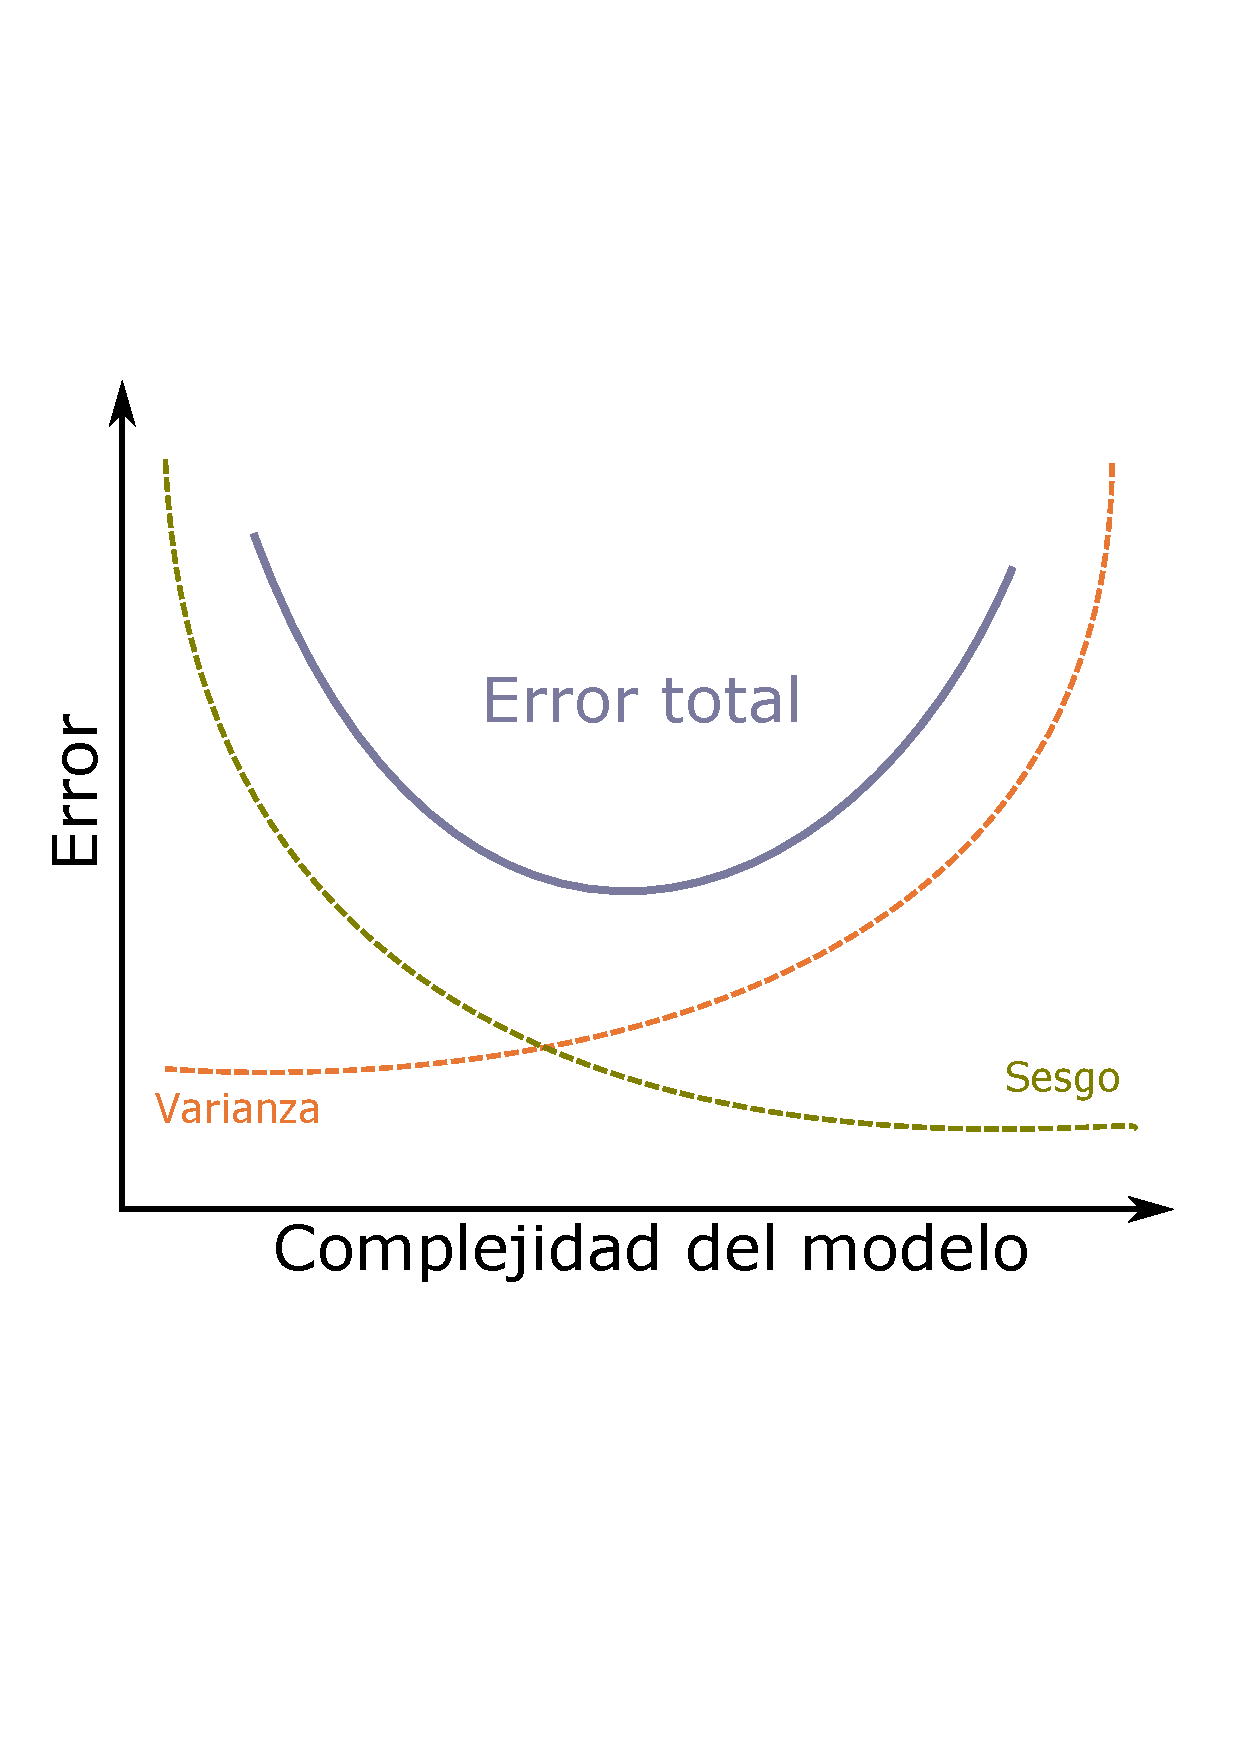
\includegraphics[width = 0.4\linewidth]{img/cap5_biasvariance.pdf}
    \caption{Tradeoff entre el sesgo y la varianza.}
\end{figure}


\subsection{Validación cruzada}

Una primera forma de elegir y evaluar un modelo fuera de muestra, consiste en particionar el conjunto de datos $\mathcal{D}$ en dos, donde con el primer conjunto se realizará el entrenamiento y con el segundo se medirá el rendimiento del modelo de acuerdo a algún criterio predefinido (por ejemplo, ECM). Con el fin de evitar posibles sesgos provocados por una partición en específico, la evaluación de desempeño se debe realizar varias veces sobre conjuntos de validación distintos. De esta forma, al promediar los rendimientos de cada partición se obtiene un rendimiento estimado fuera de muestra, lo cual permite finalmente elegir un modelo, quedándose con aquel que reporte el menor error out-sample. Las distintas formas de mezclar y particionar los datos se conocen como validación cruzada.

\subsubsection{Validación cruzada exhaustiva}

En este tipo de validación cruzada, se prueban todas las posibles permutaciones de los datos al particionar el conjunto $\mathcal{D}$. Se tienen 2 técnicas exhaustivas:

\begin{itemize}
	\item l\textbf{eave $p$ out (LpOCV):} el conjunto $\mathcal{D}$ se particiona dejando $p$ elementos para validación y los $N-p$ elementos restantes se utilizan para entrenar el modelo. Este entrenamiento y cálculo de desempeño se repite $C_p^N=\frac{N!}{(N-p)!p!}$ veces, pasando por todos los posibles conjuntos de validación de tamaño $p$.
	\item \textbf{leave one out (LOOCV):} corresponde al caso anterior con $p=1$. En este caso cada dato de $\mathcal{D}$ es utilizado como único elemento de validación mientras el resto de los datos se utiliza para entrenar.
\end{itemize}

\subsubsection{Validación cruzada no exhaustiva}

\begin{itemize}
	\item \textbf{$k$-fold:} el conjunto $\mathcal{D}$ es dividido en $k$ grupos de igual tamaño. Luego, uno de esos grupos es utilizado como validador y el resto como entranemiento. Esto se repite $k$ veces de forma de que todos los grupos sean validadores una y solo una vez.
	\item \textbf{Monte Carlo CV:} se realizan particiones binarias aleatorias de $\mathcal{D}$. Se entrena y evalúa usando el par de conjuntos creados en cada partición.
\end{itemize}

\begin{remark}
Una variante de este método es dividir el conjunto $\datos$ en 3, donde los primeros dos conjuntos son utilizados para entrenamiento y validación, mientras que el tercero (conocido como test set) es utilizado para obtener una estimación real del desempeño fuera de muestra del modelo elegido a partir de los dos conjuntos anteriores. Esto se realiza ya que al considerar únicamente el desempeño en el conjunto de validación, por lo general se sobreestima el desempeño real fuera de muestra debido a que el modelo fue elegido precisamente tomando el que reporta el menor error dentro del conjunto de validación.\\

Si bien no hay una regla estándar que indique cómo particionar el conjunto, una división usual es utilizar el 50\% para entrenamiento y 25\% para validación y test.
\end{remark}

\subsection{Selección de modelo}

Si bien la técnica de validación cruzada es bastante efectiva, tiene la limitación de requerir una gran cantidad de datos para poder realizar la partición de $\datos$. Para los casos que en los que no se cuenta con una cantidad considerable de observaciones, se requieren herramientas más sofisticadas para poder tomar una decisión acerca de qué modelo elegir. Los dos criterios más usuales corresponden al criterio de información de Akaike y al criterio de información bayesiano.\\

\subsubsection{Criterio de información de Akaike (AIC)}


Sea $\datos=(x_i)_{i=1}^N$ un conjunto de observaciones generadas por una distribución desconocida perteneciente a una familia paramétrica cuyos parámetros están en $\Theta\subset\R^d$. Bajo este modelo, se puede utilizar el estimador de máxima verosimilitud:

\begin{equation}
	\hat{\theta} = \argmax_{\theta\in\Theta} L(\theta|\datos) =  \argmax_{\theta\in\Theta} l(\theta|\datos)
\end{equation}

Una forma de evaluar el desempeño real de este estimador es mediante el \emph{riesgo de predicción}, el cual se ve reflejado en la log-verosimilitud de $\hat{\theta}$ sobre todas las posibles observaciones: $\E(l(\hat{\theta}|x))$. Dado que solo se cuenta con una cantidad finita de muestras, solo es posible obtener un riesgo empírico. El criterio de información de Akaike (AIC) busca ajustar este riesgo para obtener un estimador asintóticamente insesgado del riesgo real. Para esto, se tienen las siguientes definiciones para el estimador de máxima verosimilitud $\hat{\theta}$:

\begin{itemize}
	\item \textbf{Riesgo empírico:} $R_\datos(\hat{\theta})=-\hat{l}$, donde $\hat{l}=l(\hat{\theta}|\datos)$ es la log-verosimilitud del EMV empírico.
	\item \textbf{Riesgo real:} $R(\hat{\theta})=-\E(N\cdot l_0(\hat{\theta}))$, donde $l_0(\theta)=\E(l(\theta|x))$ corresponde a la log-verosimilitud de $\theta$ sobre todo el espacio muestral. Notar que se multiplica por $N$ ya que en el riesgo empírico no se normalizó por $N$.
\end{itemize}

Para poder obtener el $AIC$ se analizará el sesgo asintótico del riesgo empírico con respecto al riesgo real. Para esto, se utilizarán aproximaciones sobre ambos riesgos, asumiendo que a medida que $N$ crece, el EMV empírico tiende al EMV global (por LGN), por lo que el residuo de Taylor tenderá a 0.\\

Sea $\theta_0 = \argmax_{\theta\in\Theta} l_0(\theta)$ el EMV sobre todo el espacio muestral. Utilizando una aproximación de Taylor de segundo orden sobre $l_0$ alrededor de $\theta_0$:
\begin{align}
	l_0(\hat{\theta})&\approx l_0(\theta_0) + (\hat{\theta}-\theta_0)^\top \nabla l_0(\theta_0) + \frac{1}{2}(\hat{\theta}-\theta_0)^\top H_{l_0}(\theta_0) (\hat{\theta}-\theta_0)\\
	&= l_0(\theta_0) + \frac{1}{2}(\hat{\theta}-\theta_0)^\top H_{l_0}(\theta_0) (\hat{\theta}-\theta_0)
\end{align}

Donde se usó que $\nabla l_0(\theta_0)=0$ ya que $\theta_0$ es un punto crítico de $l_0$. De esta forma, se tiene una aproximación de segundo orden para el riesgo real:

\begin{equation*}
	R(\hat{\theta}) \approx -N \cdot l_0(\theta_0) - \frac{N}{2}\E\left((\hat{\theta}-\theta_0)^\top H_{l_0}(\theta_0) (\hat{\theta}-\theta_0)\right)
\end{equation*}

Por otra parte, realizando una expansión de Taylor de segundo orden sobre $\hat{l}$ alrededor de $\theta_0$:
\begin{equation}
	\hat{l} = \sum_{i=1}^N l(\hat{\theta}|x_i) \approx \sum_{i=1}^N l(\theta_0|x_i) + (\hat{\theta}-\theta_0)^\top \sum_{i=1}^N \nabla l(\theta_0|x_i) + \frac{1}{2}(\hat{\theta}-\theta_0)^\top \sum_{i=1}^N H_l(\theta_0|x_i) (\hat{\theta}-\theta_0)
\end{equation}

Usando el hecho de que $\hat{\theta}$ es punto crítico de $l(\cdot|\datos)$:
\begin{equation}
	\sum_{i=1}^N \nabla l(\theta_0|x_i) = \sum_{i=1}^N \nabla \left(l(\theta_0|x_i) - l(\hat{\theta}|x_i)\right) \approx \left(\sum_{i=1}^N \nabla l(\theta_0|x_i)\right) (\theta_0-\hat{\theta}) \approx N \E(H_l(\theta_0|x)) (\theta_0-\hat{\theta})
\end{equation}

Luego, sustituyendo en $\hat{l}$ y notando que $\sum\limits_{i=1}^N H_l(\theta_0|x_i) \approx N\E(H_l(\theta_0|x))$:

\begin{align}
	&\hat{l} \approx \sum_{i=1}^N l(\theta_0|x_i) + N(\hat{\theta}-\theta_0)^\top \E(H_l(\theta_0|x)) (\theta_0-\hat{\theta}) + \frac{N}{2}(\hat{\theta}-\theta_0)^\top \E(H_l(\theta_0|x)) (\hat{\theta}-\theta_0)\\
	&\implies \E(R_\datos(\hat{\theta})) = -Nl_0(\theta_0) + \frac{N}{2} \E\left((\hat{\theta}-\theta_0)^\top H_{l_0}(\theta_0) (\hat{\theta}-\theta_0)\right)
\end{align}

De este modo, el sesgo del riesgo empírico como estimador del riesgo real es:

\begin{equation*}
	\E(R_\datos(\hat{\theta})) - R(\hat{\theta}) = -n \E\left((\hat{\theta}-\theta_0)^\top H_{l_0}(\theta_0) (\hat{\theta}-\theta_0)\right)
\end{equation*}

Por otra parte, dado que $\sqrt{N}\left(\hat{\theta}-\theta_0\right)\approx\mathcal{N}\left(0,H_{l_0}(\theta_0)^{-1}\right)$, la forma cuadrática anterior puede ser aproximada por una distribución de Pearson: $N(\hat{\theta}-\theta_0)^\top H_{l_0}(\theta_0) (\hat{\theta}-\theta_0)\approx\mathcal{X}^2_d$, donde $\E(\mathcal{X}^2_d)=d$. De este modo,

\begin{equation}
	\E(R_\datos(\hat{\theta})) - R(\hat{\theta}) \approx -d
\end{equation}

Por lo que corrigiendo $R_\datos(\hat{\theta})$ se obtiene un estimador asintóticamente insesgado del riesgo real: $R_\datos(\hat{\theta})+d$. De esta forma, se tiene la siguiente definición:

\begin{definition}[AIC]
	Sea $M$ un modelo estadístico $d$-paramétrico y $\datos=(x_i)_{i=1}^N$ un conjunto de observaciones. El AIC del modelo (aproximado por $\datos$) se define como
	
	\begin{equation}
		AIC(M,\datos):=2d-\log\left(\hat{L}(\datos)\right)
	\end{equation}
	
	Donde $\hat{L}(\datos)$ corresponde a la verosimilitud del EMV asociado a $\datos$, es decir:
	
	\begin{equation}
		\hat{L}(\datos) = \prod_{i=1}^N p(x_i|\hat{\theta}),\text{ para } \hat{\theta} = \argmax_{\theta\in\Theta} L(\theta|\datos)
	\end{equation}
\end{definition}

\begin{remark}
El AIC corresponde al estimador asintóticamente insesgado del riesgo real multiplicado por 2. Esta ponderación es realizada por motivos históricos (Model selection and multimodel inference, Burnham \& Anderson).
\end{remark}

De acuerdo a la derivación anterior, el AIC es una medida relativa de la pérdida de información de un modelo de acuerdo a un conjunto de entrenamiento $\datos$. De esta forma, para un conjunto de posibles modelos, se debe elegir el modelo que presente el menor valor AIC ya que será el que minimice el riesgo de predicción.\\

Como se puede ver en la definición, el criterio de Akaike no se basa únicamente en la verosimilitud del modelo sino que agrega una penalización de acuerdo a la cantidad de parámetros, evitando elegir un modelo sobreajustado a los datos. 

\begin{remark}
	Una de las hipótesis de AIC es que el espacio muestral es infinito ya que se asume que el error de Taylor es despreciable. Para una cantidad finita de datos, se puede realizar una corrección del estimador dada por:
	
	\begin{equation}
		AICc(M,\datos) := AIC(M,\datos) + \frac{2d(d+1)}{N-d-1}
	\end{equation}
	
	Es importante notar que cuando $N\to\infty$ se recupera el AIC original.
\end{remark}

\subsubsection{Criterio de información bayesiano (BIC)}

Otro enfoque para la selección de modelos corresponde al criterio de información bayesiano (o criterio de Schwarz). Dada una familia de modelos $\mathcal{M}$, se define un prior $p(m)$ para cada modelo $m\in\mathcal{M}$. Además, se define un prior $p(\theta|m)$ sobre los parámetros de cada modelo. El criterio de información bayesiano (BIC) elige al mejor modelo de acuerdo a la posterior $p(m|\datos)$, la cual viene dada de acuerdo al teorema de Bayes:

\begin{equation}
	p(m|\datos)=\frac{p(\datos|m)p(m)}{p(\datos)}\propto p(\datos|m)p(m)
\end{equation}

De forma similar al criterio de Akaike, se puede calcular la verosimilitud del modelo $p(\datos|m)$ mediante aproximaciones de Taylor, probando que es independiente del prior. La derivación de $p(\datos|m)$ lleva a la siguiente definición:

\begin{definition}[BIC]
	Sea $M$ un modelo estadístico $d$-paramétrico y $\datos=(x_i)_{i=1}^N$ un conjunto de observaciones. El BIC del modelo (aproximado por $\datos$) se define como
	
	\begin{equation}
		BIC(M,\datos):= d\cdot\log(N) - 2\log\left(\hat{L}(\datos)\right)
	\end{equation}
	
	Donde nuevamente $\hat{L}(\datos)$ corresponde a la verosimilitud del EMV asociado a $\datos$.
\end{definition}

En este caso, se vuelve a elegir el modelo que presente el menor BIC. Se observa que, al igual que AIC, BIC contiene una penalización sobre el número de parámetros por lo que también evita el sobreajuste a los datos.

\begin{remark}[Stone (1977) - Shao (1997)] Para una familia de modelos, minimizar el AIC es asintóticamente equivalente a realizar LOOCV. Por otra parte, minimizar el BIC es asintóticamente equivalente a realizar leave $p$ out cross validation para

\begin{equation}
	p=\left\lfloor N\left(1-\frac{1}{\log(N)-1}\right)\right\rfloor
\end{equation}
	
\end{remark}

\begin{mdframed}[style=pendiente, frametitle={\center AIC y BIC para la regresión lineal}]

Al igual que en máxima verosimilitud, se puede considerar un modelo generativo para la regresión lineal de la forma $ y = c^\top x + \epsilon$, donde $\epsilon\sim\cN(0,\sigma^2)$ y por lo tanto, $y|x \sim \cN(y;c^\top x,\sigma^2)$. Sean $\hat{c}$ y $\hat{\sigma}^2$ los EMV del modelo (calculados en el capítulo de regresión), entonces la log-verosimilitud máxima viene dada por:
\begin{align}
	\hat{l}(\datos) &= \frac{-N}{2}\log(2\pi\hat{\sigma}^2) - \frac{1}{2\hat{\sigma}^2} \sum_{i=1}^N( y_i-\hat{c}^\top x_i)= -\frac{N}{2}\log(2\pi) - \frac{N}{2}\log(\hat{\sigma}^2) - \frac{1}{2\hat{\sigma}^2}  N\hat{\sigma}^2\\
	&= C(N) - \frac{N}{2}\log(\hat{\sigma}^2) = C(N)- \frac{N}{2}\log\left(\frac{1}{N}\text{RSS}(\datos)\right)
\end{align}	

Donde $C(N) = -\frac{N}{2}\log(2\pi) - N$ y $\text{RSS}(\datos)$ corresponde a la suma de cuadrados residuales: $\text{RSS}(\datos) := \sum_{i=1}^N \left(y_i - c^\top x_i\right)^2$. Dado que $C(N)$ es una constante independiente del modelo, puede ser omitida en la comparación de modelos, por lo tanto:

\begin{itemize}
	\item $AIC=2d-N\log(\frac{1}{N}\text{RSS}(\datos))$
	\item $BIC = d\log(N) - N\log(\frac{1}{N}\text{RSS}(\datos))$
\end{itemize}

\end{mdframed}

Si bien existen otros métodos de selección de modelo (DIC, WAIC, entre otros), estos tienen una formulación más compleja que se escapa del alcance de este curso ya que se requieren herramientas adicionales como MCMC para el cálculo de distribuciones posteriores.

\subsection{Evaluación de modelos}
Una vez elegido el mejor modelo de acuerdo a un criterio establecido (AIC o BIC), es deseable poder conocer el desempeño de dicho modelo. Existen varias formas de evaluar un modelo, una de ella podría ser simplemente evaluar la precisión de sus predicciones. A veces es natural fijarse en la precisión, como en los problemas de pronóstico. Otras veces la precisión es importante para evaluar diferentes modelos y elegir uno de ellos. En esta sección presentaremos dos maneras distintas de evaluar modelos, cada forma sirve en distintos escenarios, los cuales se discutirán a través de la predicción puntal, que resume la predicción de un conjunto de datos en una solo valor.

\subsubsection{Error cuadrático medio}

El ajuste del modelo a nuevos datos se puede resumir en una predicción puntual llamada error cuadrático medio, el cual está definido por:

\begin{equation}
MSE(\theta) = \frac{1}{n}\sum_{i=1}^N (y_i-\mathbb{E}(y_i|\theta))^2
\end{equation}

o su versión ponderada:

\begin{equation}
MSE(\theta) = \frac{1}{n}\sum_{i=1}^N \frac{(y_i-\mathbb{E}(y_i|\theta))^2}{\mathbb{V}\text{ar}(y_i|\theta)}
\end{equation}

Esta forma de medir el error tiene la ventaja de ser fácilmente computable e interpretable, pero no es apropiada para modelos que están lejos de la distribución normal.

\subsubsection{log-densidad predictiva o log-verosimilitud}
Otra forma de realizar esta evaluación es utilizando el estadístico \emph{log-densidad preditiva} $\log p(y|\theta)$ el cual es proporcional a error cuadrático medio si el modelo es normal con varianza constante. Estudiaremos el caso de un solo punto, para luego extrapolar a más de un punto.\\

\textbf{Predictive accuracy para un punto:} sea $f$ el modelo real, $y$ las observaciones (es decir, una realización del dataset $y$ de la distribución $f(y)$), y llamaremos $\tilde{y}$ a la data futura o un dataset alternativos que podemos ver. El ajuste predictivo out-of-sample para un nuevo punto $\tilde{y}_i$ está dado por:

\begin{equation}
\log p_{\text{post}}(\tilde{y}_i) = \log \mathbb{E}[p(\tilde{y}_i|\theta)] = \log \int p(\tilde{y}_i|\theta)p_{\text{post}}(\theta)d\theta
\end{equation}

\textbf{Promedio de las distribuciones para un punto:} al tener un dato nuevo $\tilde{y}_i$ entonces se puede calcular el la log-densidad predictiva (elpd, por su sigla en inglés) para el nuevo punto:
\begin{align}
\notag \text{elpd} & = \mathbb{E}_f[\log p_{\text{post}}(\tilde{y}_i)]\\
& = \int \log p_{\text{post}}(\tilde{y}_i) f(\tilde{y}_i)d\tilde{y}
\end{align}

\textbf{Promedio de las distribuciones para datasets futuros:} como usualmente, no se tiene solo un punto, se debe realizar la suma sobre el conjunto de puntos, calculando así la log-densidad predicitiva puntual (elppd, por su sigla en inglés).

\begin{align}
\text{elppd} & = \sum_{i=1}^N \mathbb{E}_f[\log p_{\text{post}}(\tilde{y}_i)]
\end{align}

En la práctica, como siempre se tiene la distribución de todos los modelos y la expresión anterior requiere de esto, se suele calcular el estadístico sobre una estimación de un modelo $\hat{\theta}$ (como por ejemplo, el máximo de la función de verosimilitud):

\begin{align}
\text{elppd}|\hat{\theta} & = \sum_{i=1}^N \mathbb{E}_f[\log p_{\text{post}}(\tilde{y}_i|\hat{\theta})]
\end{align}

Finalmente, una última extensión de este estadístico es cuando se puede tener \emph{draws} de la posterior, es decir, tenemos $\{ \theta^s\}_{s=1}^S$, entonces el lppd computado es:

\begin{equation}
\text{computed lppd} = \sum_{i=1}^N \left( \frac{1}{S} \sum_{s=1}^S p(y_i|\theta^s)\right)
\end{equation}


\subsection{Promedio de modelos}
Hay veces que no queremos elegir un solo modelo, puesto que quizás nos interesan las estimaciones de dos o más modelos. Para estos casos, se puede utilizar la técnica de \emph{model averaging}, la cual consiste en utilizar una combinación lineal de distintos modelos.\\

Sea $\mathcal{M}$ un conjunto de modelos donde cada modelo $m\in\mathcal{M}$ tiene asociada una distribución $\mu_m$ sobre el espacio muestral. Un promedio de modelos $\hat{\mu}$ es una combinación convexa de los modelos de $\mathcal{M}$, es decir:

\begin{equation}
\hat{\mu} = \sum_{m\in \mathcal{M}} c(m) \mu_m
\end{equation}

Donde los pesos $\left(c(m)\right)_{m\in\mathcal{M}}\subset\R_+$ cumplen que $\sum_{m\in \mathcal{M}} c(m) = 1$.\\

La principal dificultad para elegir los pesos, está en que se debe asegurar que la suma de los pesos sea unitaria y que estos sean todos positivos. Una forma de asegurar esto es aplicar una función $f$ positiva sobre una función $g$ (\emph{score}) que evalúe el modelo, de modo que:

\begin{equation}
\sum_{m\in \mathcal{M}} (f\circ g)(m) > 0
\end{equation}

De esta forma, se pueden definir los pesos mediante normalización:

\begin{equation}
c(s) = \frac{(f\circ g)(s)}{\sum_{m\in \mathcal{M}} (f\circ g)(m)}
\end{equation}

Para la función $g$ se pueden utilizar los criterios AIC o BIC ya que entregan una evaluación del desempeño relativo del modelo. Por otra parte, usando $f(x)=\exp(x)$ los pesos $\left(c(m)\right)_{m\in\mathcal{M}}$ vienen dados por la función softmax:



\begin{align}
c_{AIC}(s) = \frac{\exp\{ \frac{1}{2} \text{AIC}(s)\}}{\sum_{m\in \mathcal{M}} \exp\{ \frac{1}{2} \text{AIC}(m)\}} & & c_{BIC}(s) = \frac{\exp\{ \frac{1}{2} \text{BIC}(s)\}}{\sum_{m\in \mathcal{M}} \exp\{ \frac{1}{2} \text{BIC}(m)\}}
\end{align}
